\documentclass{article}

\usepackage[margin=1in]{geometry}
\usepackage{spverbatim}
\usepackage{graphicx}

\begin{document}
	
\title{ESOF 322 - Homework 2}
\author{Nathan Stouffer and Kevin Browder}

\maketitle
\newpage

\section*{Part A}

Pictured below is our class diagram. \\\\
\begin{figure}[h]
	\centering
	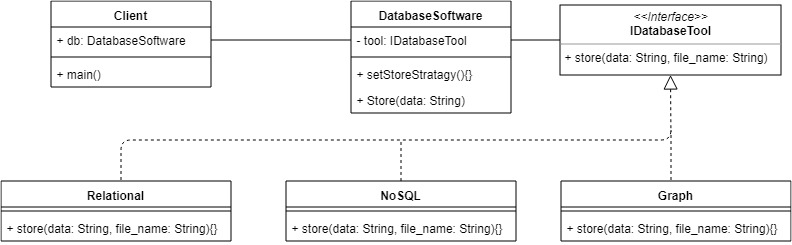
\includegraphics[scale=.5]{class-diagram.jpg}
\end{figure}

\newpage

\section*{Part B}

\subsection*{Code}

\begin{spverbatim}
	/**
	* interface with a method called store
	*/
	public interface IDatabaseTool {
		
	    public void store(String data, String file_name);
		
	}
\end{spverbatim}

\newpage

\begin{spverbatim}
	import java.io.File;
	import java.io.FileWriter;
	import java.io.IOException;
	
	/**
	* class that implements a dummy database software
	* 
	* A client can switch between different storage tools
	* using the setStorageStrategy method
	* 
	* The data will be written to the same file, regardless
	* of what storage tool is chosen
	* 
	*/
	public class DatabaseSoftware {
		
	    // instance of database tool interface
	    private IDatabaseTool tool;
	    // output file name
	    String file_name = "database-output.out";
		
	    /**
	    * constructor for DatabaseSoftware object
	    * default database tool is set to relational
	    */
	    DatabaseSoftware(){ 
	        // create empty file
	        createEmptyFile(file_name);
			
	        // dummy output line
	        System.out.println("Created Database Software object\nDefault tool is Relational");
			
	        // instantiate tool with Relational constructor
	        this.tool = new Relational();
	    }
		
	    /**
	    * method to store the data using the current store strategy
	    * @param data 
	    */
	    public void Store(String data){ tool.store(data, this.file_name); }
		
	    /**
	    * method to set a new store strategy
	    * @param temp 
	    */
	    public void setStoreStrategy(IDatabaseTool temp){ this.tool = temp; }
		
	    /**
	    * method to create an empty output file
	    * @param file_name 
	    */
	    private void createEmptyFile(String file_name){
	        File file = new File(file_name);
	        try{
	            FileWriter fw = new FileWriter(file);
	            fw.write("");
	            fw.close();
	        }
	        catch (IOException e){ System.err.println("IO error"); }
	    }
		
	}
\end{spverbatim}

\newpage

\begin{spverbatim}
	import java.io.FileWriter;
	import java.io.File;
	import java.io.IOException;
	
	/**
	* class that stores data using the Relational tool
	* (via that table store method)
	* 
	* class Relational implements the IDatabaseTool interface
	*/
	public class Relational implements IDatabaseTool {
		
	    /**
	    * constructor with a dummy output line to tell user
	    * that they are now using the relational tool
	    */
	    Relational(){ System.out.println("\nYou are using the Relational database tool"); }
		
	    /**
	    * method to store the data using the table store method
	    * @param data
	    * @param file_name 
	    */
	    public void store(String data, String file_name){
	        fileOutput(data, file_name);
	        System.out.println("Stored data using table store method");
	    }
		
	    /**
	    * method to write the data to an output file
	    * @param data
	    * @param file_name 
	    */
	    private void fileOutput(String data, String file_name){
	        File file = new File(file_name);
	        try{
	            FileWriter fw = new FileWriter(file, true);
	            fw.write(data);
	            fw.close();
	        }
	        catch (IOException e){ System.err.println("IO error"); }
	    }
		
	}
\end{spverbatim}

\newpage

\begin{spverbatim}
	import java.io.File;
	import java.io.FileWriter;
	import java.io.IOException;
	
	/**
	* class that stores data using the NoSQL tool
	* (via that document store method)
	* 
	* class Relational implements the IDatabaseTool interface
	*/
	public class NoSQL implements IDatabaseTool {
		
	    /**
	    * constructor to output dummy line to tell user
	    * that they are now using the NoSQL tool
	    */
	    NoSQL(){ System.out.println("\nYou are using the NoSQL database tool"); }
		
	    /**
	    * method to store data using document store method
	    * @param data
	    * @param file_name 
	    */
	    public void store(String data, String file_name){
	        fileOutput(data, file_name);
	        System.out.println("Stored data using document store method");
	    }
		
	    /**
	    * method to write the data to an output file
	    * @param data
	    * @param file_name 
	    */
	    private void fileOutput(String data, String file_name){
	        File file = new File(file_name);
	        try{
	            FileWriter fw = new FileWriter(file, true);
	            fw.write(data);
	            fw.close();
	        }
	        catch (IOException e){ System.err.println("IO error"); }
	    }
	}
\end{spverbatim}

\newpage

\begin{spverbatim}
	import java.io.File;
	import java.io.FileWriter;
	import java.io.IOException;
	
	/**
	* class that stores data using the Graph tool
	* (via that node store method)
	* 
	* class Relational implements the IDatabaseTool interface
	*/
	public class Graph implements IDatabaseTool {
		
	    /**
	    * constructor to output dummy line to tell user
	    * that they are now using the NoSQL tool
	    */
	    Graph(){
	         System.out.println("\nYou are using the Graph database tool");
	    }
		
	    /**
	    * method to store data using the node store method
	    * @param data
	    * @param file_name 
	    */
	    public void store(String data, String file_name){
	        fileOutput(data, file_name);
	        System.out.println("Stored data using node store method");
	    }
		
	    /**
	    * method to write the data to an output file
	    * @param data
	    * @param file_name 
	    */
	    private void fileOutput(String data, String file_name){
	        File file = new File(file_name);
	        try{
	            FileWriter fw = new FileWriter(file, true);
	            fw.write(data);
	            fw.close();
	        }
	        catch (IOException e){ System.err.println("IO error"); }
	    }
	}
\end{spverbatim}

\newpage

\subsection*{Output}

Our console output is shown below. The console output consists of print statements from methods. In addition to these print statements, the string "A line of data" is written to a file whenever the \emph{Store()} method is called on a DatabaseSoftware object.

\begin{figure}[h]
	\centering
	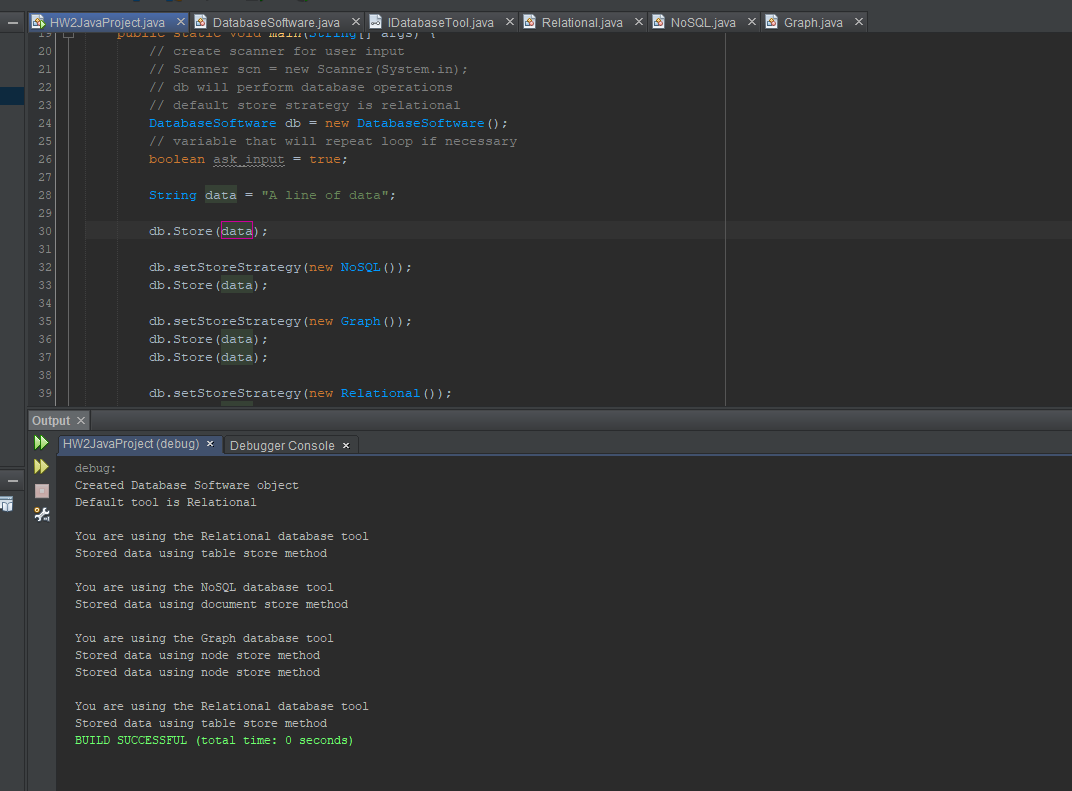
\includegraphics[scale=0.75]{console-output.png}
\end{figure}

\newpage

\section*{Part C}

Pictured below is our sequence diagram. The sequence diagram pictures how our code switches between two strategies. \\\\ 
\begin{figure}[h]
	\centering
	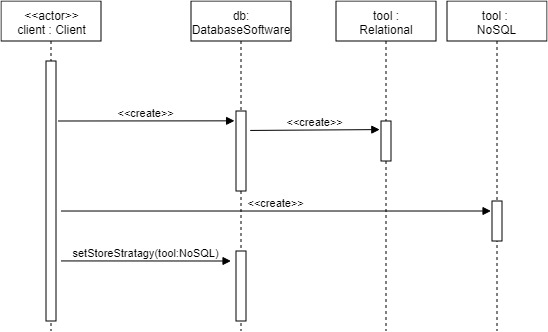
\includegraphics[scale=0.5]{sequence-diagram.jpg}
\end{figure}
	
\end{document}